\documentclass[a4paper, 12pt]{article}

\usepackage{forloop}
\usepackage{graphicx}
\usepackage{subcaption}
\usepackage{amsmath}
\usepackage{url}
\usepackage{tikz}

\let\vec\mathbf  % Make vectors bold, instead of arrow

\author{Thorvald M. Ballestad}
\title{Assignment 1 - TFY4235\\
  Fractal drum}

\begin{document}
\maketitle

\begin{abstract}
  Investigating the eigenmodes of a fractal drum.
  Is it possible to say something about the shape of a drum from its eigenfrequencies?
\end{abstract}

\section{Introduction}
In this project we investigate the eigenmodes of a fractal drum.
The infinte fractal shape is approximated by a finite recursion.
The wave equation is solved in fourier space using a finite element method.
We are interested in finding out what recursion level we are able to achieve and how accurately we can estimate the fractal dimension of the drum based on the numerical solutions to the eigenfrequencies.

\section{Theory}
The relevant theory is given in the exercise text\cite{exercise}.
The most important parts are repeated here.

The fractal is a Koch fractal, more specifically the Minkowski Sausage variant\cite{wiki:Koch}.
The iteration for creating this fractal is transforming each line segment into a square wave, shown in figure \ref{fig:fractal-transform}.
\begin{figure}[h]
  \centering
  \begin{tikzpicture}
    \draw (0,0) -- ++(4,0);
    \draw[->] (4.3, 0) -- (4.7, 0);
    \draw (5,0) -- ++(1,0) -- ++(0,1) -- ++(1,0) -- ++(0, -2) -- ++(1,0) -- ++(0,1) -- ++(1,0);
  \end{tikzpicture}
  \caption{One iteration of the fractal generation.}
  \label{fig:fractal-transform}
\end{figure}
Beginning with a square, apply the iteration for each segment.
For each new segment, apply the iteration recursively.
The square is denoted as level 0, after the first iteration we are at level 1 and so on.

The fractal is placed on a grid.
For this grid we will define a grid constant $\delta$.
$\delta=1$ corresponds to a grid where the distance between grid points is the same as the length of the shortest line segment on the fractal.
For $\delta=2$, there are two grid points for each shortest line segment, and so on.

The wave equation we want to solve, in Fourier space, is
\begin{subequations}
  \label{eq:helm}
  \begin{align}
    -\nabla^2 U(\vec{r}, \omega) &= \frac{\omega^2}{v^2} U(\vec{r}, \omega), &&\text{in } \Omega\\
    U(\vec{r}, \omega) &= 0, &&\text{on } \partial \Omega.
  \end{align}
\end{subequations}
Discretice $U(\vec{r})$ as $U_{x,y}$, where $x$ and $y$ are integers, and $U_{x,y} = U(xh\hat{x} + yh\hat{y})$, where $h$ is the distance between grid points.
For the discrete laplacian, we will use five point and nine point stencil.
That is, central finite difference in two dimensions at second and fourth order defined as \cite{wiki:DifferenceCoef}\cite{wiki:FivePoint}:

\begin{subequations}
  \label{eq:stencil}
  \begin{align}
  h^2\nabla_5^2 U_{x,y} &=
  U_{x+1,y} + U_{x-1,y} + U_{x,y+1} + U_{x,y-1} - 4 U_{x,y}\\
  h^2\nabla_9^2 U_{x,y} &=
  \frac43 U_{x+1,y} + \frac43 U_{x-1,y} + \frac43 U_{x,y+1} + \frac43 U_{x,y-1}\\
  & -\frac{1}{12}U_{x+2,y} - \frac{1}{12}U_{x-2,y} - \frac{1}{12}U_{x,y+2} - \frac{1}{12}U_{x,y-2}\nonumber\\
  &- 5 U_{x,y}\nonumber,
  \end{align}
\end{subequations}
where the subscripts on the $\nabla^2$-operator denotes five and nine point stencil respectively.

As described in \cite{exercise} the Weyl-Berry conjecture predicts that
\begin{equation}
  \Delta N(\omega) = \frac{A}{4\pi} \omega^2 - N(\omega)
\end{equation}
scales as $\omega^d$, where $d$ is the fractal dimension of the drum.
The fractal dimension of our fractal, when recursion level $l\rightarrow\infty$, is $3/2$\cite{exercise}.
This quantity can therefore be used for numerical validation.

\section{Method}
\subsection{Generating the fractal}
The generation of the fractal structure is implementet quite naievly.
For example, the array of points is not pre-allocated, but appended during each loop-cycle.
The number of points for a given level is easy to calculate, so this would be a simple thing to fix, but as it is not time consuming at all, the naive method is kept.
The fractal points are stored as integers.
See \ref{sec:lattice}.

\begin{figure}[h]
  \centering
  \begin{subfigure}[b]{.49\textwidth}
      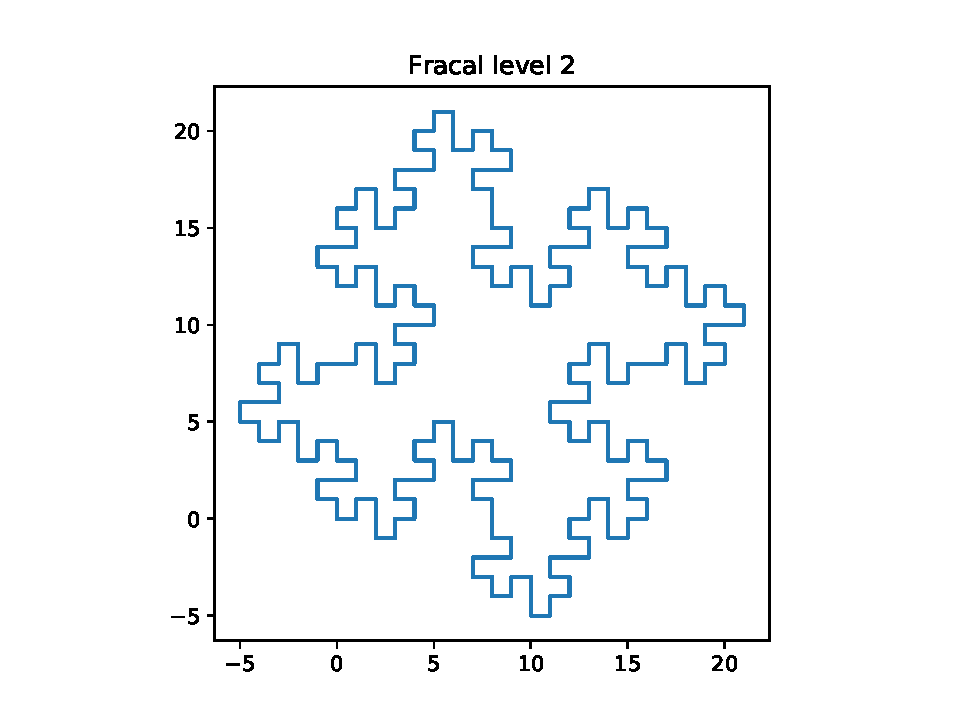
\includegraphics[width=\textwidth]{media/fractal_l2}
  \end{subfigure}
  \begin{subfigure}[b]{.49\textwidth}
      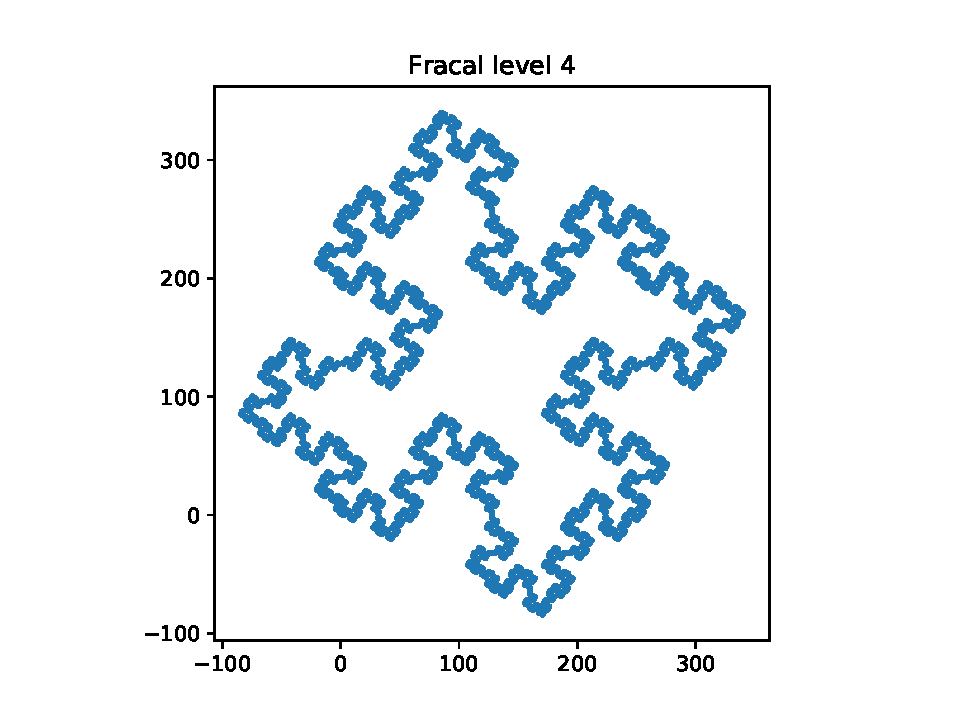
\includegraphics[width=\textwidth]{media/fractal_l4}
  \end{subfigure}
  \caption{Fractal for $l=2$ and $l=4$.}
\end{figure}

\subsection{The lattice\label{sec:lattice}}
The lattice is a 2D array of integers.
Each array element has a value that corresponds to either inside, outside, or on the border of the fractal.
The lattice constant $\delta$ is implemented in such a way that the shortest segment on the fractal, correspond to $\delta$ steps on the lattice.
Ie. if $\delta=1$, there are no points on the lattice between the start and end point of the line segment on the fractal.

\subsection{Inside or outside -- determination of inner points\label{sec:insideoutside}}
There are two methods implemented in the program for determining if a point is inside or outside the fractal.
The only assumption about the structure that the methods makes, is that every line segment is either vertical or horizonal, and not diagonal.

The first method is a breadth first-type search.
Given a point that we know is inside the structure, add its four cardinal points -- above, below, right, and left -- into a list.
Visit each of the points in the list.
For each of these points that are not border points, append their cardinal points to the list.
Continue this process until the list is empty.
Notice that the list is processed FILO.
A FIFO process would give a depth first search.
One could argue that this method is not complete, as it requires one starting point inside the structure.
However, if one hits the ``edge'' of ones region, without hitting a border point, one knows that the starting point was not inside the structure, and thus the method is complete.
Also, in the problem at hand we know trivially that the center point of our area is inside the curve.
This method will be called middle out.

The second method is based on counting border crossings.
For each point in our area, move in one direction, here left, and count the number of border crossings before reaching the end of the area.
If it is odd, the point is inside, if it is even the point is outside.
The complication is how to count border crossings for a discretized curve.
Here, it is done as follows:
The grid constant must be at least two.
Without this, the problem is not solvable -- one can easily construct cases where it would be ambiguous where the curve goes.
When scanning, in this case left, check for each point if it is a border point.
If it is, check if the point below it is also a border point.
If that is the case, count it as a border crossing.
This method will be called scan.

On a level 4 fractal with grid constant 2, the performance of the two methods is shown in table \ref{tab:insideoutside}.

\begin{table}[h]
  \centering
\begin{tabular}{lrrr}
  Method& Time[s]& Allocations& Memory[MiB]\\
  \hline
  Middle out& 0.069& 788K& 32\\
  Scan& 3.33& 54M& 835
\end{tabular}
\caption{Performance of two methods for determining if points are inside or outside.
  Found for level 4 with grid constant 2.
  The methods are described in \ref{sec:insideoutside}
  \label{tab:insideoutside}}
\end{table}

\subsection{Calculation of eigenmodes}
We convert \eqref{eq:helm} into an eigenproblem on matrix form.
This is done by converting $U_{x,y}$ into a 1D array $U'$ containing all the innner points of the fractal.
A corresponding matrix, representing $\nabla^2$ also made.
The programatic challenge here is constructing the matrix, or more precisely mapping our structure onto $U'$ and then find the entries in our matrix that match the operator defined in  \eqref{eq:stencil}.

There are two aspects of the solution worth mentioning.
When discussing the lattice, it was mentioned that each point is an integer representing either inside, outside or border.
More specifically -1 represents outside and zero represents border.
Any positive integer is inside.
Each inner point is given an unique positive integer, representing that points index in $U'$.
This way, we have a direct lookup from the grid to $U'$.
One also need a lookup from $U'$ to the grid.
An array of the same dimension as $U'$, with tuples with the grid coordinates does this.

The second aspect worth mentioning is the datastructure of the eigenmatrix.
This matrix is extremely sparse.
Therefore it is  stored in compressed sparse column format, which is the standard sparse format in Julia.\\

Arpack is used to solve the system.

\section{Results and discussion}
\subsection{Eigenmodes and eigenfrequencies}
Level five is the highest recursion level for which I am able to solve the system.
The eigenmatrix is then a $983041\times 983041$ matrix, which takes 85MB of memory.
The limitations then is obviously not the size of the matrix, but the memory Arpack requires to solve the system.

Table \ref{tab:eigenvalues} shows the first ten eigenvalues, calculated at level five with grid constant 2.
The first ten eigenmodes are shown in figure \ref{fig:eigenmodes}.
The eigenmodes were calculated at level four with grid constant 2, using the five point stencil.

\begin{table}[h]
  \centering
  \begin{tabular}{cc}
    Five point& Nine point\\
    \hline
    5.752& 5.753\\
    8.625& 8.628\\
    8.625& 8.628\\
    8.791& 8.795\\
    8.839& 8.842\\
    9.200& 9.202\\
    9.200& 9.202\\
    10.768& 10.771\\
    11.533& 11.537\\
    11.866& 11.869\\
  \end{tabular}
  \caption{The 10 lowest eigenfrequencies, $\omega/v$, calculated at level five with grid constant two.
    Five point and nine point refers to whether five point or nine point stencil was used.
  \label{tab:eigenvalues}}
\end{table}

\newcounter{mode}
\begin{figure}[p]
  \centering
\forloop{mode}{1}{\value{mode}<10}{
    \begin{subfigure}[b]{.30\textwidth}
      \includegraphics[width=\textwidth]{media/modes/mode_\arabic{mode}.pdf}
    \end{subfigure}
    \stepcounter{mode}
    \begin{subfigure}[b]{.30\textwidth}
      \includegraphics[width=\textwidth]{media/modes/mode_\arabic{mode}.pdf}
    \end{subfigure}
}
\caption{The first 10 eigenmodes\label{fig:eigenmodes}}
\end{figure}


\subsubsection{Approximation of the Laplacian operator}

\subsection{Estimation of fractal dimension}
As described calculation of fractal dimension can be used for numerical validation.
The first one thousand calculated values for $\Delta N(\omega)$ is shown in figure \ref{fig:fractal_dimension}.
The values were found for recursion level four of the fractal and with grid constant three.
The values have distinct ``drops'' in an otherwise smooth curve, at $\omega \approx 0.07$ and $\omega \approx 0.15$.
Because of this, the fitted curve is calculated using two different intervals.
The first uses all the calculated values, while the second uses only the values up to the first ``drop''.
They are denoted ``Fitted curve'' and ``Fitted curve for first section'' respectively, and the calculated values $d$ and $d_2$.


\begin{figure}[ht]
  \centering
  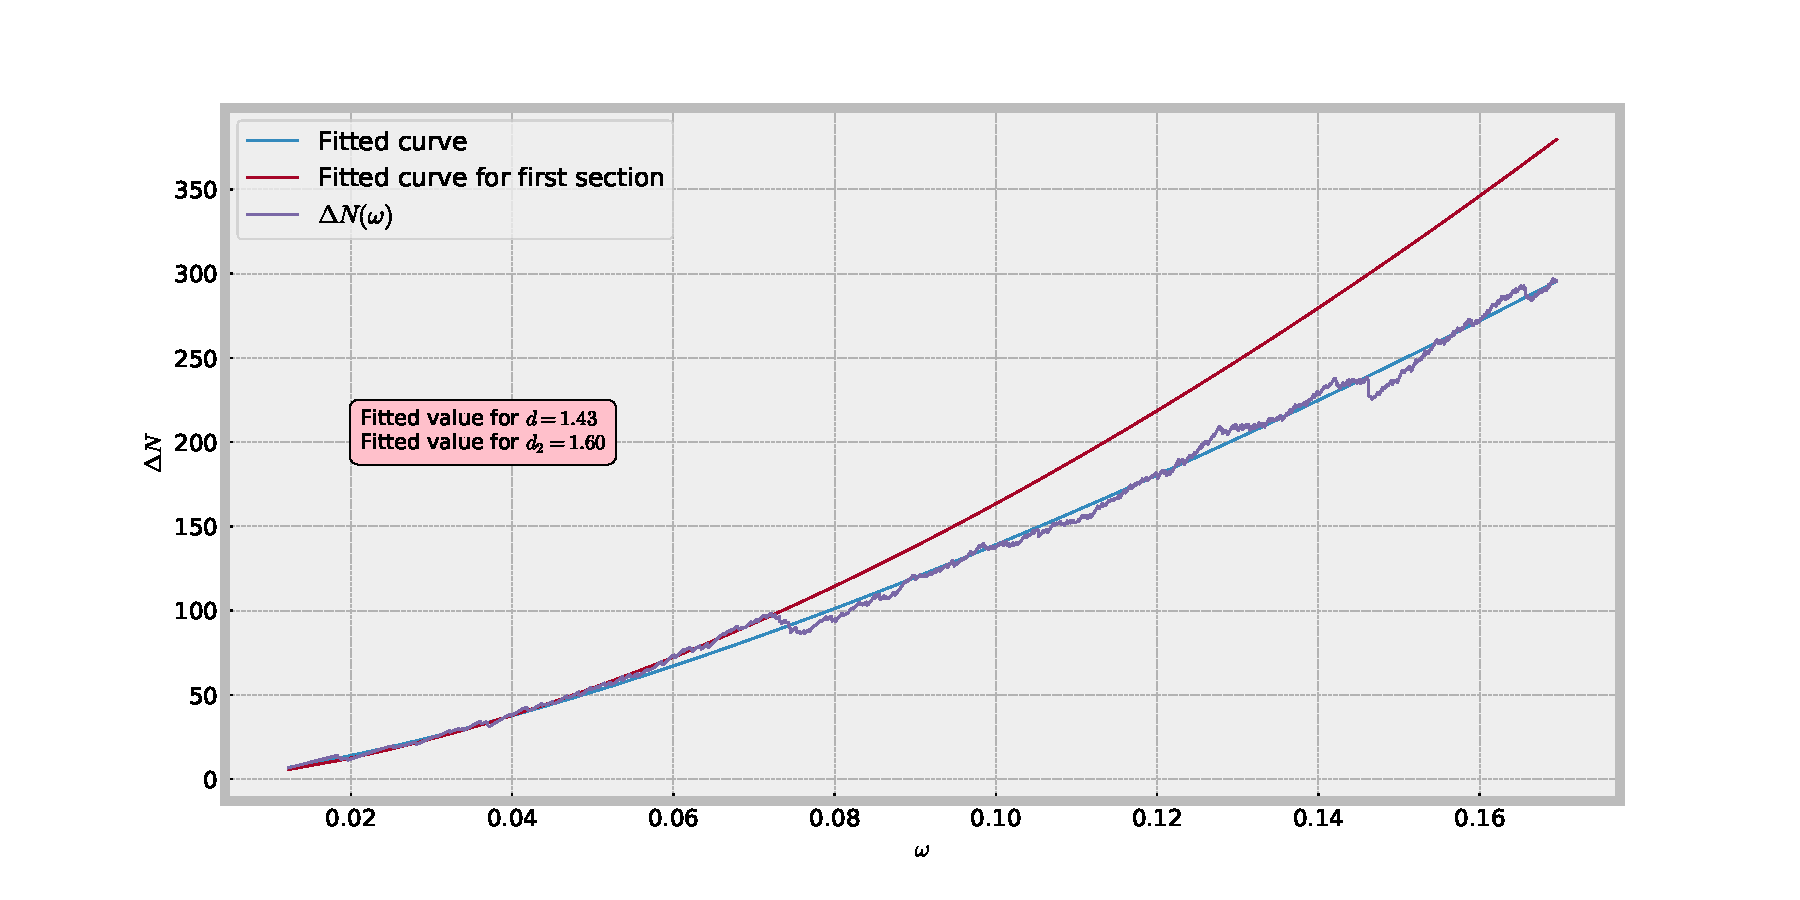
\includegraphics[width=0.75\textwidth]{media/fractal_dimension_delta_N_values_level_4_grid_constant_3_num_modes_999}
  \caption{The first one thousand values of $\Delta N(\omega) = \frac{A}{4\pi} \omega^2 - N(\omega)$, where $N(\omega)$ is the integrated density of states.
    Calculated using recursion level four and grid constant three.
    The two fitted curves were found using all the points and using only the points until the first ``drop''.
    Theoretically the value of $d$ should be 1.5.
    The calculated values for $d$ is 1.43 and 1.60 respectively.
  \label{fig:fractal_dimension}}
\end{figure}

\subsection{Future extensions of the simulation}

\begin{thebibliography}{9}
\bibitem{exercise} TFY4235/FY8904: Computational Physics (spring 2020) Assignment1: Vibrations of Fractal Drums. Ingve Simonsen, \emph{Department of Physics, NTNU}. \url{http://web.phys.ntnu.no/~ingves/Teaching/TFY4235/Assignments/TFY4235_Assignment_01.pdf}. Retrieved Mar 13. 2020.

\bibitem{wiki:Koch} Wikipedia, Koch Snowflake, \url{https://en.wikipedia.org/wiki/Koch_snowflake}. Retrieved Mar 6. 2020.

\bibitem{wiki:DifferenceCoef} Wikipedia, Finite difference coefficient, \url{https://en.wikipedia.org/wiki/Finite_difference_coefficient}. Retrieved Mar 11. 2020.
\bibitem{wiki:FivePoint} Wikipedia, Five-point stencil, \url{https://en.wikipedia.org/wiki/Five-point_stencil}. Retrieved Mar 11. 2020.
\end{thebibliography}
\end{document}
